\documentclass[11pt]{article}
\usepackage{../../latex/preamble}

\usepackage{multicol}
\usepackage{media9}
\newtheorem*{viralthm}{Viralteoremet}
\newcommand{\abs}[1]{|#1|}
\begin{document}
  % make title page
\begin{titlepage}
  \newcommand{\HRule}{\rule{\linewidth}{0.5mm}}
  \center
  \textsc{\LARGE Universitetet i Oslo}\\[1.5cm] % Name of your university/college
  \textsc{\Large }\\[0.5cm] % Major heading such as course name
  \textsc{\large FYS3150}\\[0.5cm] % Minor heading such as course title
  \HRule \\[0.4cm]
  { \huge \bfseries N-body simulering}\\[0.4cm]
  \HRule \\[1.5cm]
  \Large \emph{Skrevet av:}\\
  Lyder \textsc{Rumohr Blingsmo} (k.nr. 2) og Bendik \textsc{Samseth} (k.nr. 27)\\[3cm]
  {\large \today}\\[3cm]
  \vfill
\end{titlepage}

\tableofcontents
\begin{abstract}
I denne rapporten utvikler vi en N-body modell. Det vil si et system av
$N$ masser som vekselvirker kun ved gravitasjon. Spesielt studerer vi kollaps
av et slik system når alle partiklene begynner i ro. Vi sammenligner 
stabiliteten til to forskjellige løsningsmetoder, RungeKutta4 og VelocityVerlet,
ved å kikke på energibevaring i systemet. 
Alt materiale som har blitt referert er tilgjengelig
 på Github~\cite{github-repo}. 
\end{abstract}

\begin{multicols}{2}



\section{Innledning}
Vi skal se på et stjernekluster med $N$ partikler. I vår modell tenker
vi oss at hver partikkel representerer en eller noen få stjerner. Vi
skal også anta at gravitasjon er den eneste kraften som virker:

\begin{align}
 \vec F = -\frac{GM_1M_2}{r^3}\vec r.\
\end{align}

Her er $G$ gravitasjonskonstanten, $M_i$ er massene og $r$ er avstanden mellom dem. 
Denne antagelsen er god under forutsetningen av at $r$ er relativt
stor slik at  ingen kontaktkrefter gjør seg gjeldene. Vi bruker
Newtons andre lov, og får differensialligningene 

\begin{align} \label{eq:a_i}
a_i = \sum_{j \neq i} \frac{GM_j}{{|\vec{r_i} - \vec{r_j}|}^2} , \ \ \
  i = 1,2, \cdots N 
\end{align}

der $a_i$ er akselerasjonen til masse $i$. Dette er et system av
ordinære differensialligninger, noe vi kan løse ved å anvende
numeriske metoder. I denne rapporten ser vi på RungeKutta4 og Velocity-Verlet.

\subsection{Kort om RungeKutta4~\small{\cite{RK4}}}
Metoden antar en funksjon på formen 
\begin{align*}
\dot{y} = f(t, y), \quad y(t_0) = y_0,
\end{align*}

som i vårt tilfelle er gitt ved \eqref{eq:a_i} med 

\begin{align*}
\dot y = \dot{v_i} = a_i 
\end{align*}
Vi trenger initialbetingelser for hastighet,
\begin{align*}
 v_i(t_0) = v_{i,0}.
\end{align*}
Vi velger en steglengde $h>0$ og definer 

\begin{align*}
y_{n+1} &= y_n + \tfrac{h}{6}\left(k_1 + 2k_2 + 2k_3 + k_4 \right)\\
t_{n+1} &= t_n + h \\
\end{align*}
der vi har
\begin{align*}
k_1 &= f(t_n, y_n), \\
k_2 &= f(t_n + \tfrac{h}{2}, y_n + \tfrac{h}{2} k_1), \\
k_3 &= f(t_n + \tfrac{h}{2}, y_n + \tfrac{h}{2} k_2), \\
k_4 &= f(t_n + h, y_n + hk_3).
\end{align*}

Vi gjentar så metoden en gang til for 

\begin{align*}
\dot{x_i} = v_i.
\end{align*}
I realiteten er det mulig å vektorisere prosessen slik at vi løser
både hastigheten og posisjonen til alle partiklene samtidig.

\subsection{Kort om Velocity-Verlet~\small{\cite{Velocity-Verlet}}}
\label{sec:om-VV}
Vi anvender også Velocity-Verlet på \eqref{eq:a_i}. Denne metoden fungerer for tilfeller der 
akselerasjonen ikke er en funksjon av hastigheten. 
Algoritmen for metoden er gitt som følger:

\begin{enumerate}
\item Regn ut: \begin{align*}
\vec{v}\left(t + \tfrac12\,\Delta t\right) = \vec{v}(t) + \tfrac12\,\vec{a}(t)\,\Delta t\ 
\end{align*}


\item Finn så: \begin{align*} \vec{r}(t + \Delta t) = \vec{r}(t) + \vec{v}\left(t + \tfrac12\,\Delta t\right)\, \Delta t \end{align*}


\item Regn ut: \begin{align*} \vec{a}(t + \Delta t) 
\end{align*} fra \eqref{eq:a_i} med posisjonen $ \vec{r}(t + \Delta t) $


\item Til slutt: \begin{align*} \vec{v}(t + \Delta t) = \vec{v}\left(t + \tfrac12\,\Delta t\right) + \tfrac12\,\vec{a}(t + \Delta t)\Delta t \end{align*}
\end{enumerate}

\subsection{Initialisering av systemet}
\label{sec:init-av-system}
Vi kan selv velge fritt starttilstanden til systemet vårt. Vi velger å
begynne med $N$ objekter fordelt uniformt innenfor en sfære med
radius $R_0=20 ly$ (light years). Objektene gir vi en tilfeldig masse ved å la massene
følge en Gaussisk fordeling med snittverdi $10M_\odot$ og standardavik
på $M_\odot$. Her er $M_\odot$ solmassen. Vi lar alle starte i ro. 

Av disse startbetingelesene er det en del som trenger noe ekstra
oppmerksomhet\footnote{Det som følger er i stor grad en oversettelse
  av et skriv laget av H. T. Ihle som ble sendt ut via epost (ikke
  listet som en referanse fordi den ikke kan vises til noe sted).}. Det er ikke helt fullstendig trivielt å lage uniformt
fordelte koordinater innenfor en sfære. Problemet er at hvis vi lar
objektene være uniformt fordelt i $r$, så vil vi ende med en mye
større tetthet rundt midten av sfæren. Og hvis vi fordeler objektene
uniformt i $\theta$ vil tettheten blir mye større rundt polene. 

Vi løser dette ved å bruke at volumelementet skal være det samme i
alle koordinatsystemer. Vi innfører koordinatene $u, v, w \in [0,1]$
og kobler disse koordinatene mot (i rekkefølge) $r,\theta$ og
$\phi$. Vi kan da skrive 
\begin{align*}
  r^2\sin\theta dr d\theta d\phi = (abc)dudvdw
\end{align*}
der $A=abc$ er en konstant. Separerer vi likningen for hvert par av
koordinater får vi likningene 
\begin{align*}
  r^2dr = adu,\ \ \sin\theta d\theta = bdv,\ \ d\phi = cdw
\end{align*}
Begynner vi med den siste og enkleste får vi 
\begin{align}
  d\phi = cdw\Rightarrow \phi = 2\pi w
\end{align}
der vi har brukt at $\phi=2\pi$ må svare til $w=1$. Samme
fremgangsmåte for $r$ og $\theta$ gir
\begin{align}
  r &= R_0 \sqrt[3]{u}\\
  \theta &= \arccos(1-2v).
\end{align}
Vi får de kartesiske koordinatene ved vanlig overgang fra sfæriske
koordinater:
\begin{align*}
  x = r\sin\theta\sin\phi\\
y = r\sin\theta\sin\phi\\
z = r\cos\theta.
\end{align*}


\subsubsection{Forventninger}
Disse initialbetingelsene blir samlet kalt sfærisk
kald-kollaps~\cite{cold-collapse}. I grensen der $N\rightarrow\infty$,
med en konstant massetetthet $\rho_0$, vil vi se at legemene kollapser
sammen i en singulæritet og danner et kontinuerlig fluid. Det kan
vises at dette vil skje etter en tid~\cite{project5-exercise}
\begin{align}
  \tau_\text{crunch} = \sqrt{\frac{ 3\pi }{ 32G\rho_0 }}\label{eq:t-crunch}.
\end{align}
Dette blir dermed en veldig naturlig tidsenhet, og vi måler alle tider
i antall $\tau_\text{crunch}$. 

Vi vil derimot ikke forvente å se en singulæritet i vår
simulering. Dette er fordi vi ser på punktmasser som kun vekselvirker
gjennom gravitasjon, i tillegg til at vi selvsagt må begrense oss til
en endelig verdi for $N$. Hva vi derimot vil forvente å se er at noen
partikler blir slynget ut av systemet (unnslipper), mens resten blir
værende i en eller annen form for bane rundt et felles massesenter. 

\section{Implementering og testing}
Hovedprogrammet er skrevet i C++, mens vi har gjort dataanalysen i Python.
Alle programmer er tilgjengelig på Github~\cite{github-repo}. 

\subsection{Klassesystem}
Vi har to klasser. Én objektklasse 'Body' som inneholder med posisjon, fart 
og masse for et gitt legeme. Den andre klassen er 'Universe' og initialiseres
med et gitt antall 'Body'-objekter. Denne klassen inneholder mange metoder,
som f.eks. \texttt{Universe::energy} for å regne ut energien til systemet, og 
\texttt{Universe::solve\_RK4} eller \texttt{Universe::solve\_Verlet} for å løse systemet
for en gitt tid.

\subsection{Løsningsmetoder}
Selve implementasjonen av løsningsmetodene er noe innviklet. Dette
kommer av at vi har et system av to ordinære differensialligninger,
hver med tre koordinater. Altså har vi egentlig seks diff.likninger
som skal løses samtidig. Metodene som vi har skissert tidligere endrer
ikke form, men det kan bli litt vanskelig å holde styr på alt
sammen. Derfor skal vi gå nokså grundig i gjennom hvordan disse
metodene er implementert. Dvs., vi gjør dette for Runge-Kutta;
Velocity-Verlet er løst på en analog måte. RK4 er implementert i
\texttt{Universe} slik som vist i vedlegg \ref{lst:solver-RK4}. 

Vi begynner med å definere flere $N\times 7$ matriser. Dette svarer til
en rad per legeme, der kolonnene er de tilhørende verdiene av (i rekkefølge) $x,y,z,v_x,v_y,v_z$
og $M$. For eksempel matrisen $y_i$ er på formen
\begin{align*}
  y_i = \begin{pmatrix}
    x_1&y_1&z_1&v_{x_1}&v_{y_1} &v_{z_1} & m_1\\
    x_2&y_2&z_2&v_{x_2}&v_{y_2} &v_{z_2} & m_2\\
    \vdots&&\ddots&&&&\vdots\\
    x_N&y_N&z_N&v_{x_N}&v_{y_N} &v_{z_N} & m_N\\
  \end{pmatrix}
\end{align*}

Til å begynne med fyller vi $y_i$ med data fra den initielle tilstanden til systemet.
Vi går så inn i tidsløkken. Her brukes en funksjon
\texttt{derivative(y\_i, a\_i, n\_bodies)} som gjør at matrisen $a_i$ fylles med de
deriverte verdiene av matrise $y_i$. Det vil si at posisjonen i $y_i$
får tilsvarende element i $a_i$ satt som hastigheten, og hastigheten i
$y_i$ blir tilsvarende satt til akselerasjonen i $a_i$. 

\begin{align*}
  a_i = \begin{pmatrix}
    v_{x_1}&v_{y_1} &v_{z_1}&a_{x_1}&a_{y_1} &a_{z_1} & m_1\\
    v_{x_2}&v_{y_2} &v_{z_2}&a_{x_2}&a_{y_2} &a_{z_2} & m_2\\
    \vdots&&\ddots&&&&\vdots\\
    v_{x_N}&v_{y_N} &v_{z_N}&a_{x_N}&a_{y_N} &a_{z_N} & m_N\\
  \end{pmatrix}
\end{align*}

Med denne fremgangsmåten følges så algoritmen for Velocity-Verlet som
er skissert i seksjon \ref{sec:om-VV}. Samme type tanke blir brukt for
å implementere Rungekutta4.


\subsection{Test av 2body-system}
For å forsikre oss om at algoritmen fungerer begynner vi med å simulere
et system med kun to legemer. I et slikt enkelt system er det lett å 
sammenligne resultatene med ens egen intuisjon av systemet. Det finnes
også en analytisk løsning. I figur \ref{fig:2body} kan vi se resultatet 
av en kjøring. Vi ser at banene er ellipsoider, slik vi forventer for
to-legeme-systemet. 

\end{multicols}

\begin{figure}[!h]
  \centering
  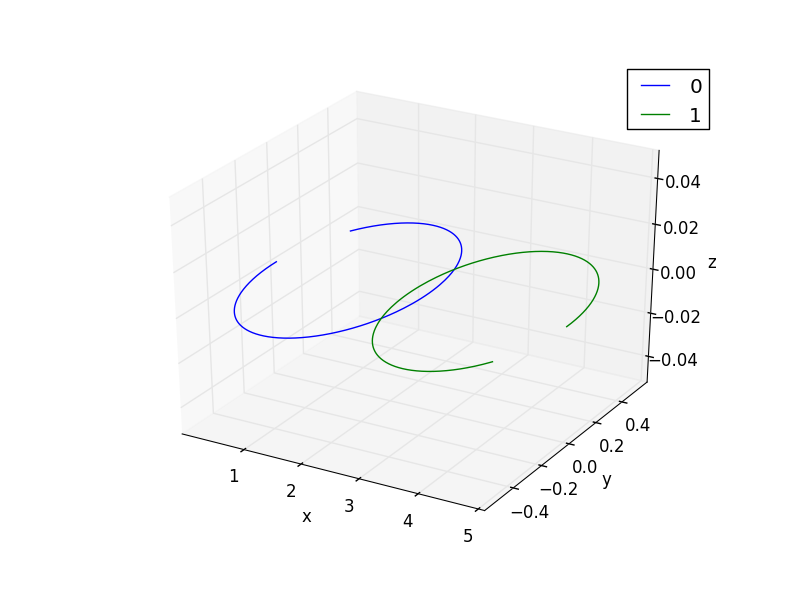
\includegraphics[scale=0.4]{../fig/2body.png}
  \caption{\label{fig:2body} En figur som viser to legemer sin bane, når eneste
    kraft som virker på dem er gravitasjon. Partikkel 0 starter i 
    punktet $(0,0,0)$ og partikkel 1 i $(5,0,0)$. De har hastigheter 
    henholdsvis $\vec{v} = (0, -0.1, 0) $ og $\vec{v} = (0, 0.1, 0)$  }
\end{figure}


\begin{multicols}{2}

\subsection{Første test av N-body}
\label{sec:forste-test-epsilon}
Det er ikke alltid lett å sjekke om en løsning gir mening. Vi begynner med
å animere systemet \footnote{Tilgjengelig på \cite{github-repo} under navnet
animate\_pos.py}, og ser fort at det skjer noe rart når massene kommer veldig
nærme hverandre. Noen legemer blir 'skutt' ut i stor fart. Dette kommer som
vi ser fra uttrykket \eqref{eq:a_i} av at akselerasjonen,$a$, blir veldig
stor når $r \rightarrow 0$.
Som en korreksjon til dette legger vi til et feilledd i kraften

\begin{align}
F_{mod} = -\frac{GM_1M_2}{r^2 + \epsilon},
\end{align}

der $\epsilon$ gjør at $F_{mod}$ ikke går i lufta når $r^2 \rightarrow 0$. Vi 
rettferdiggjør denne korreksjonen ved at masser i den virklige
verden aldri vil komme så nærme hverandre fordi de ikke er punktmasser.
Til å begynne med setter vi $\epsilon = 10^{-3}$, som vi senere vil se gir
gode resultater. Denne verdien er funnet etter prøving og feiling. 
$\epsilon > 10^{-3}$ gir oss en uønsket stor dempning i kraften, og 
$\epsilon < 10^{-3}$ gir fort samme problem som vi begynte med, deling på
veldig små tall. Vi merker oss at $\epsilon = 10^{-3} {ly}^2$ (light years) er et veldig 
stort tall, til sammenligning er $R_{solar}^2 \sim 10^{-15} {ly}^2$. 

\subsection{Energibevaring}
Selv om animasjoner alltid er flott, tenker vi det kan være lurt å ha en mer
'matematisk' test på systemet vårt. Dette gjør oss også mer egnet til
å gjøre en kvalitativ vurdering av hvilken av de løsningsmetodene som er best.
I et slikt ideelt system med bare 
gravitasjon, en konservativ kraft, er det naturlig å se på energibevaring. Vi får
energien

\begin{align}
E_{p} = - \sum_{i = 1}^{N} \sum_{j = i+1}^{N} \frac{GM_jM_i}{{||\vec{r_i} - \vec{r_j}||}} \\
E_{k} = \sum_{i} \frac{1}{2}M_i|\vec{v_i}|^2 \\
E_{tot} = E_{p} + E_{k}
\end{align}

I tabell \ref{tab:RKvsVV} ser vi en sammenligning av energibevaringen til 
våre to metoder. Rungekutta bruker lengre tid uten betydelig bedre 
energibevaring. For å spare kjøretid velger vi derfor å bruke 
Velocity-Verlet. Tabellen viser oss også at vi trenger ganske små tidssteg,
$h \leq 10 ^{-4}$ for å få god energibevaring.

\end{multicols}

\begin{table*}[h]
\centering
\caption{En tabell som sammenligner relativ energiendring for de to metodene
RungeKutta4 og VelocityVerlet. Energiendringen regnes ut fra systemet starter
i ro ved $t_0 = 0$ til $T$ for to forskjellige steglengder
$h$.  Kjøretiden, $T$, måles i enhet $\tau_{crunch}$. Ideelt sett vil vi ha $\Delta E = 0$. Vi ser Rungekutta bruker omtrent dobbelt så lang tid for en gitt h,
uten å gi noe særlig bedre presisjon.}
\label{tab:RKvsVV}
\vspace{0.5cm}
\begin{tabular}{ccccc}
Kjøreparametre $(T, log(h))$ & $(0.79,-3)$ & $(0.79,-4)$ & $(2.5,-3)$ & $(2.5,-4)$ \\
\hline 
Energiendring og tidsforbruk,$(E,\Delta t)$ RK4 & $(2.4E-01, 006.6)$ & $(2.8E-03, 046.7)$ & $(6.6E-01, 011.1)$ & $(2.2E-02, 120.8)$ \\
Energiendring og tidsforbruk,$(E,\Delta t)$ VV & $(4.9E-01, 001.9)$ & $(2.9E-03, 027.5)$ & $(9.1E-01, 005.7)$ & $(5.1E-03, 058.6)$ \\
\hline
\end{tabular}
\end{table*}

\begin{multicols}{2}
\subsection{Utskytning av partikler}
Rundt tidspunktet $\tau_{crunch}$ og i en stund etter vil partikler skytes ut
av det opprinnelige kuleskallet. Dette er partikler som ikke vil
være en del av vår likevektstilstand, og vi ønsker derfor å ha muligheten
til å se bort fra dem. Men hvordan kan vi identifisere en partikkel
som er skutt ut? Vi vet at en partikkel med $E_i > 0$ har $E_K > |E_p|$, og
vil derfor unnslippe galaksehopen. Dette viser seg derimot å være ustabilt. Se
f.eks. figur \ref{fig:energivariasjon} der vi kan se at den gjennomsnittlige
energien varierer lite, selv om den 'lokale' energien noen ganger gjør et hopp.
 På grunn av denne lokale numeriske ustabiliteten ser vi oss nødt til å gjøre
noe mer robust enn kun å se på energien. Vi observerer at en utskutt 
partikkel alltid vil forsvinne mot 'det fjerne', og derfor at 
$r_{utskutt} > R_0$. Vi bestemmer oss derfor for at i vårt program har
en utskutt partikkel ikke \emph{bare} positiv energi, $E > 0$, men befinner seg også
utenfor kuleskallet vi begynte med. 

I programmet vårt fjerner vi de utskutte
partiklene ved å sette massen og hastighetene til null, og å gjemme dem bort i et 'hjørne'. 


\subsection{Definisjon av likevekt}
En konsekvens av at vi fjerner partikler er at energien ikke lenger er bevart
gjennom hele simuleringen. Til gjengjeld får vi en veldig fin måte å definere
likevekt på. Det følger naturlig fra forrige avsnitt at likevektstilstanden
er når ingen flere partikler fjernes, det vil si energien ikke forandrer seg
betydelig lenger.

\end{multicols}
\begin{figure}[!ht]
  \centering
  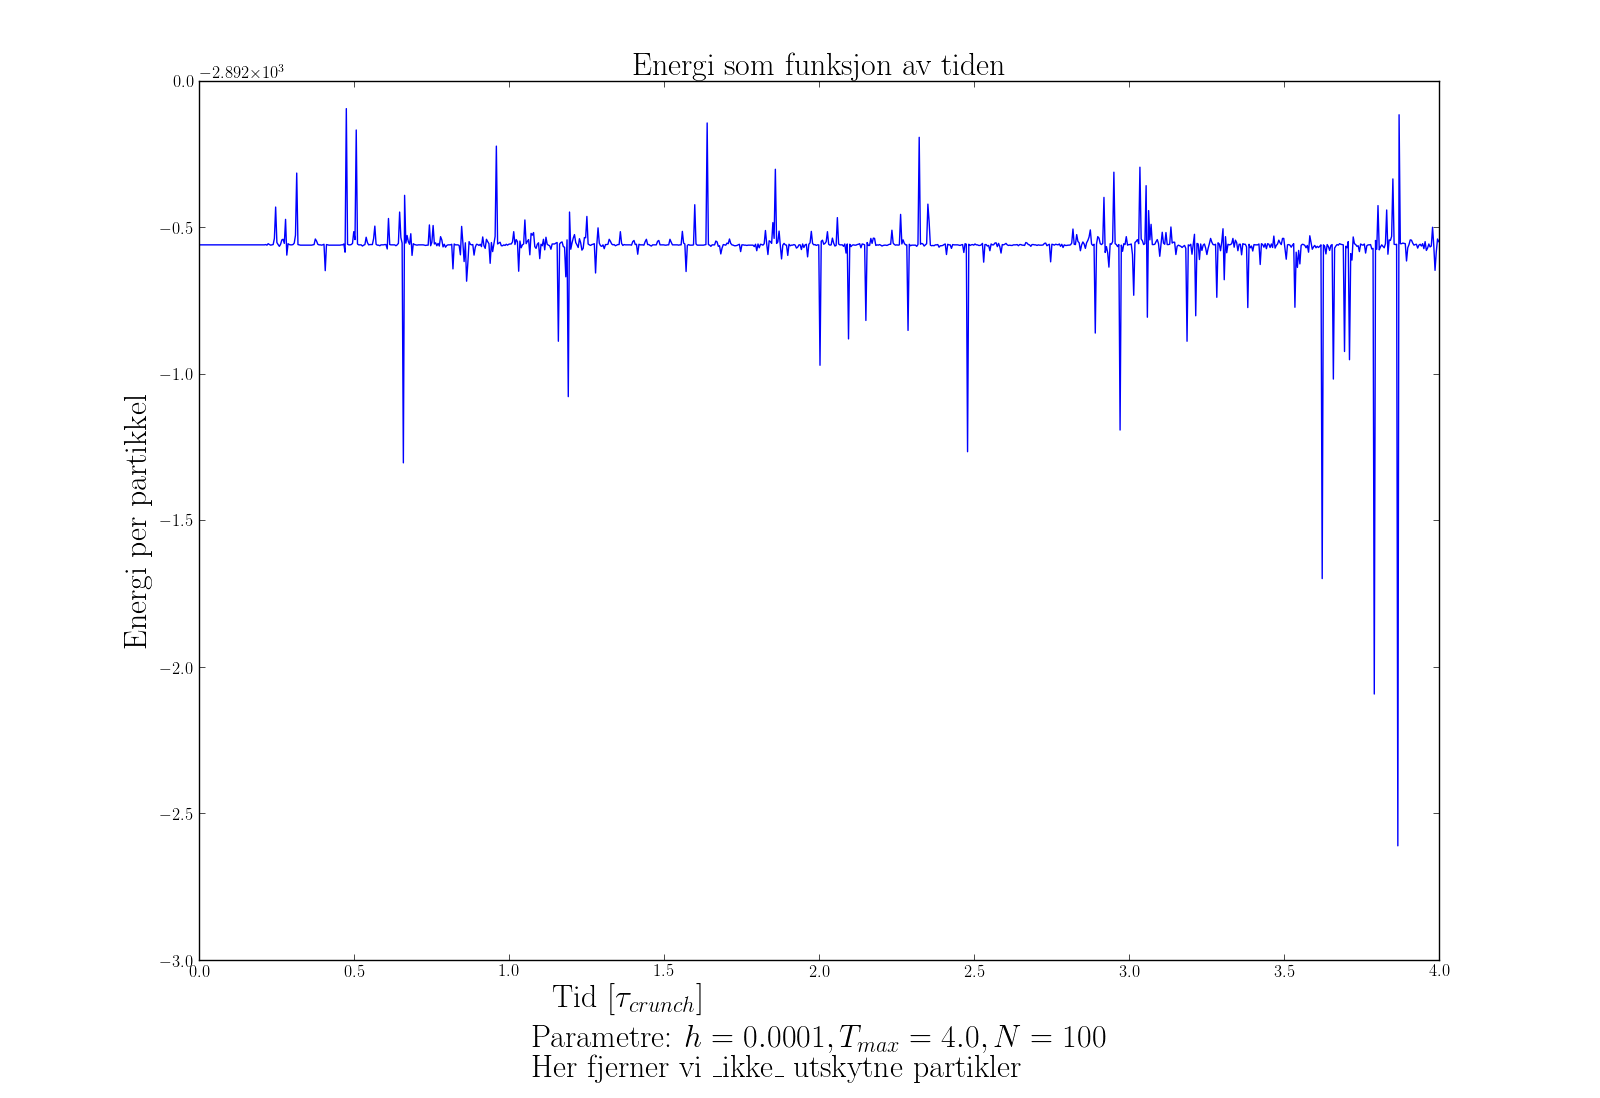
\includegraphics[width=\textwidth]{../fig/energivariasjon.png}
  \caption{\label{fig:energivariasjon} En figure som viser  }
\end{figure}

% \includemedia[
%   width=0.4\linewidth,
%   height=0.3\linewidth,
%   activate=pageopen,
%   addresource=../fig/animation.mp4,
%   flashvars={source=../fig/animation.mp4}
% ]{}{VPlayer.swf}

\cleardoublepage
\begin{multicols}{2}

\section{Resultater}
Vi har som nevnt i seksjon \ref{sec:init-av-system} simulert et system
av $N$ partikler uniformt fordelt i en sfære med radius $R0$. Vi har
laget noe animasjoner som viser tidsforløpet til
systemet~\cite[\texttt{project5/fig/}]{github-repo}. Fra animasjonene
ser vi følgende:
\begin{enumerate}
  \item Alle partiklene begynner i ro, og beveger seg sakte inn mot
    origo.
  \item Alle partiklene blir most sammen i sentrum av systemet.
  \item Partiklene spretter tilbake igjen, noen helt ut av systemet,
    andre i mindre grad.
  \item Vi står til slutt igjen med et redusert antall partikler som
    ser ut til å bevege seg noen lunde stabilt rundt i massesenteret.
\end{enumerate}

\subsection{Likevekt}
Det ser altså ut som om systemet en stund etter $\tau_\text{crunch}$
stabiliserer seg i en slags likvekt. For å se litt mer kvantitativt på
dette kan vi se på energien til systemet som en funksjon av tid. Figure
\ref{fig:energi-vs-tid-med-utskytning} viser dette. 

\end{multicols}
\begin{figure}[ht!]
  \centering
  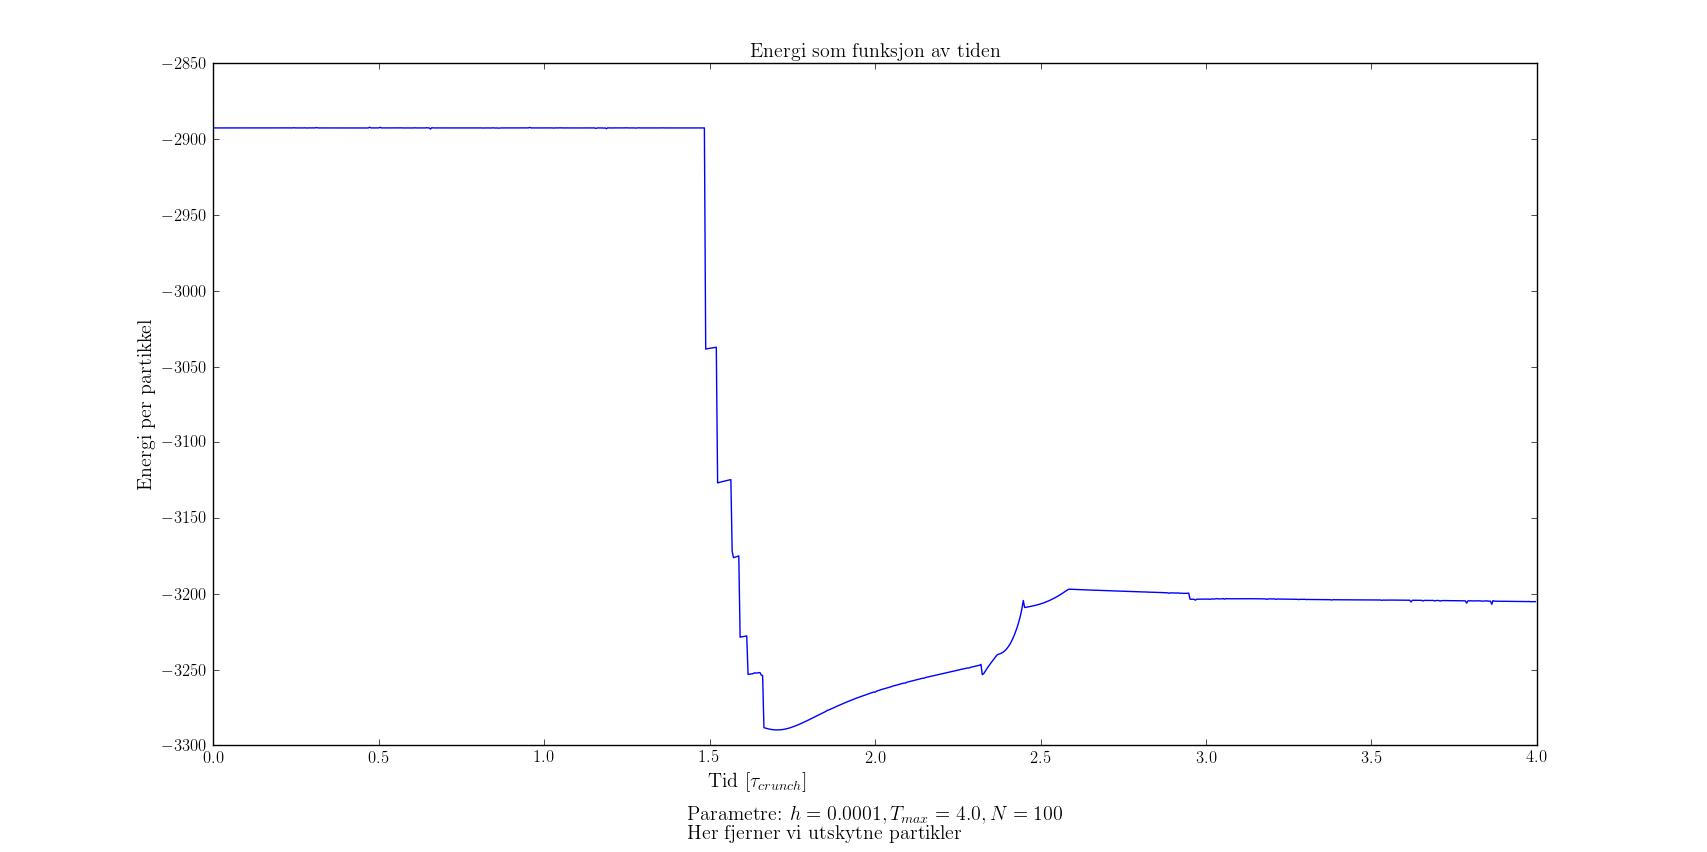
\includegraphics[width=\textwidth]{../fig/energy_plot_with_ejection.png}
  \caption{\label{fig:energi-vs-tid-med-utskytning} Systemets
    totalenergi som funksjon av tid med masseutskytelse. Vi legger
    særlig merke til at en liten tid etter $\tau_\text{crunch}$ får vi
  en voldsom reduksjon i energien til systemet. Vi ser så at etter en
  tid ser energien ut til å stabilisere seg på et lavere nivå.}
\end{figure}
\begin{multicols}{2}
Vi ser fra figuren at energien er konstant i en tid litt større enn
$\tau_\text{crunch}$. Deretter ser vi en veldig bratt, og stykkvis
nedgang i energien. Dette er fordi alle partiklene har blitt most
sammen ved tiden $\tau_\text{crunch}$, hvor noen har fått positiv
totalenergi og beveger seg ut fra systemet. Grunnen til at nedgangen
ser ut til å komme forsinket på figuren er på grunn av at vi også
krever at partikkelen også er utenfor radiusen $R_0$, noe som selvsagt
tar en viss tid. Deretter bruker systemet litt tid på å stabilisere
og etter omtrent $t = 2.5\,\tau_\text{crunch}$ ligger energien igjen
flatt. 

Grunnen til at totalenergien blir mer negativ når vi tar ut partiklene
følger logisk av at vi bare tar ut partikler som har netto positiv
energi. Tar vi vekk disse blir totalen åpenbart mer negativ. 

I figur
\ref{fig:prosentandel-utskutte} kan vi se hvordan prosentandelen
av partiklene som blir skutt ut endrer seg som funksjon av N. 

\end{multicols}
\begin{figure}[ht!]
  \centering
  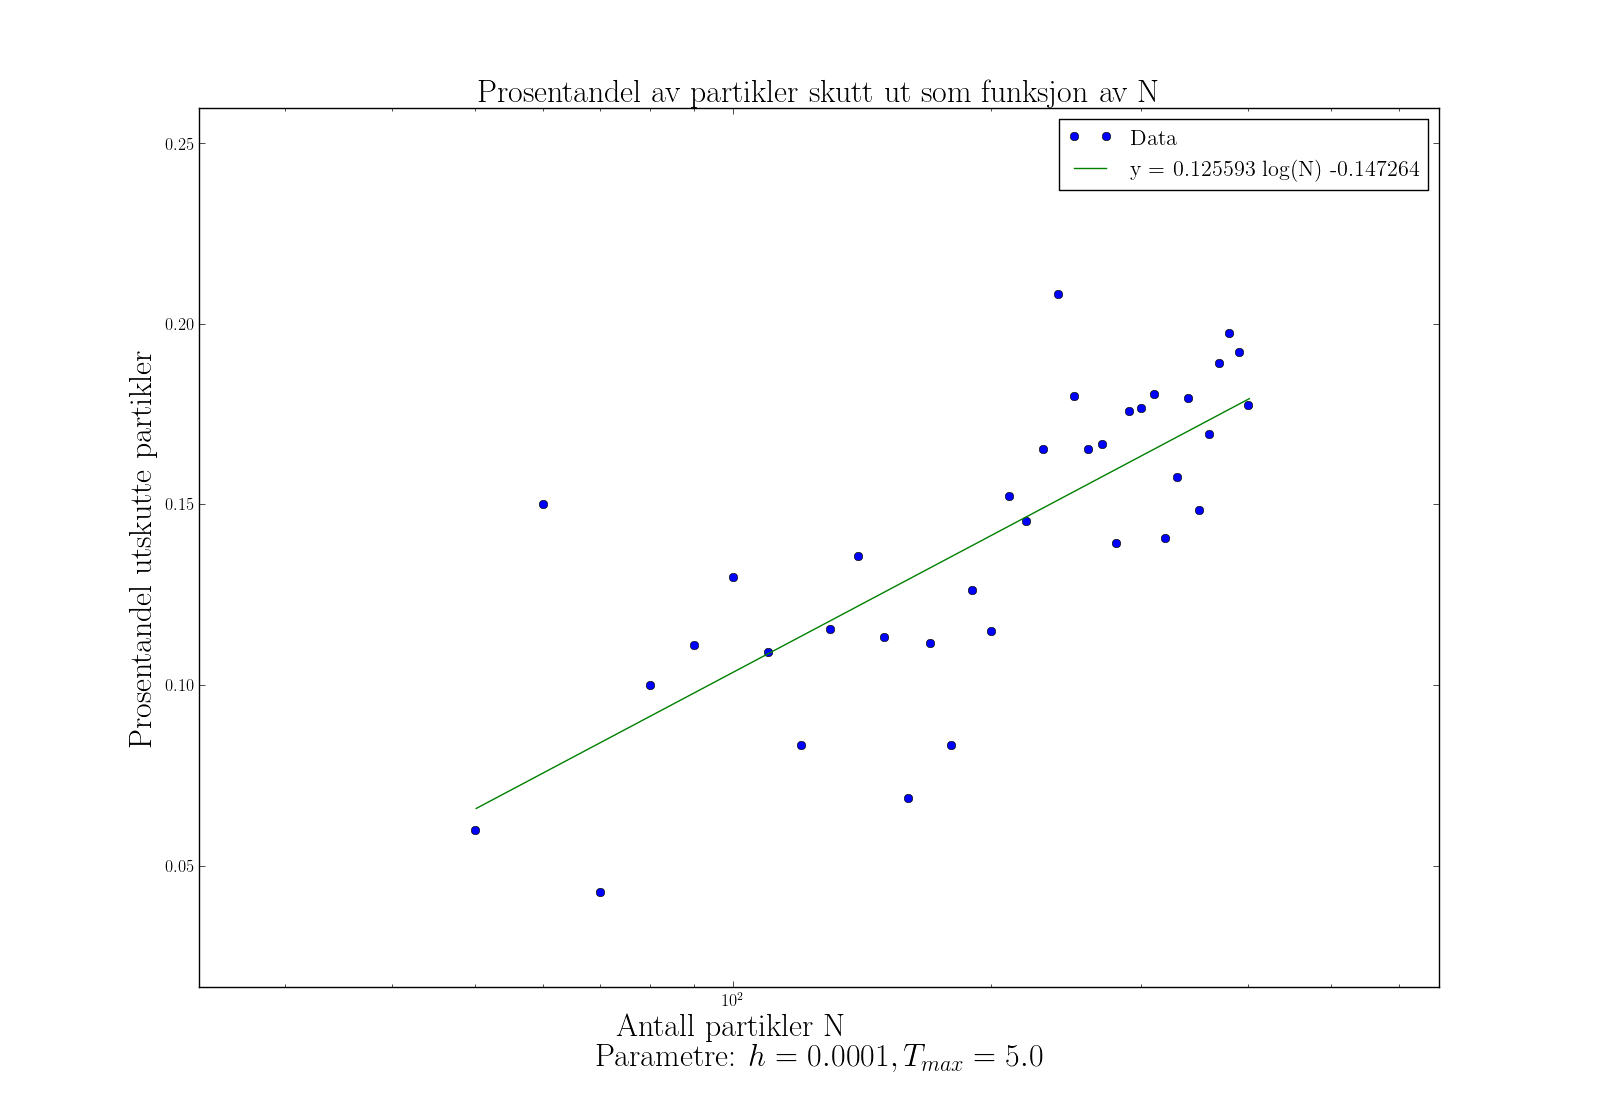
\includegraphics[width=\textwidth]{../fig/prosentandel.png}
  \caption{\label{fig:prosentandel-utskutte} Systemets
    totalenergi som funksjon av tid med masseutskytelse. Vi legger
    særlig merke til at en liten tid etter $\tau_\text{crunch}$ får vi
  en voldsom reduksjon i energien til systemet. Vi ser så at etter en
  tid ser energien ut til å stabilisere seg på et lavere nivå.}
\end{figure}
\begin{multicols}{2}

\subsubsection{$N$-avhengighet}
Vi kan lure på hvordan dette endrer seg med $N$. I figur
\ref{fig:energy-many-N} ser vi tidsforløpet til systemenergien for
forskjellige antall partikler. Først kan vi merke oss at alle
systemene begynner å miste partikler etter omtrent samme tid (en liten
tid etter $\tau_\text{crunch}$), og at alle ser ut til å bruke samme
tid på å nå et nytt stabilt energinivå. 

\end{multicols}
\begin{figure}[!ht]
  \centering
  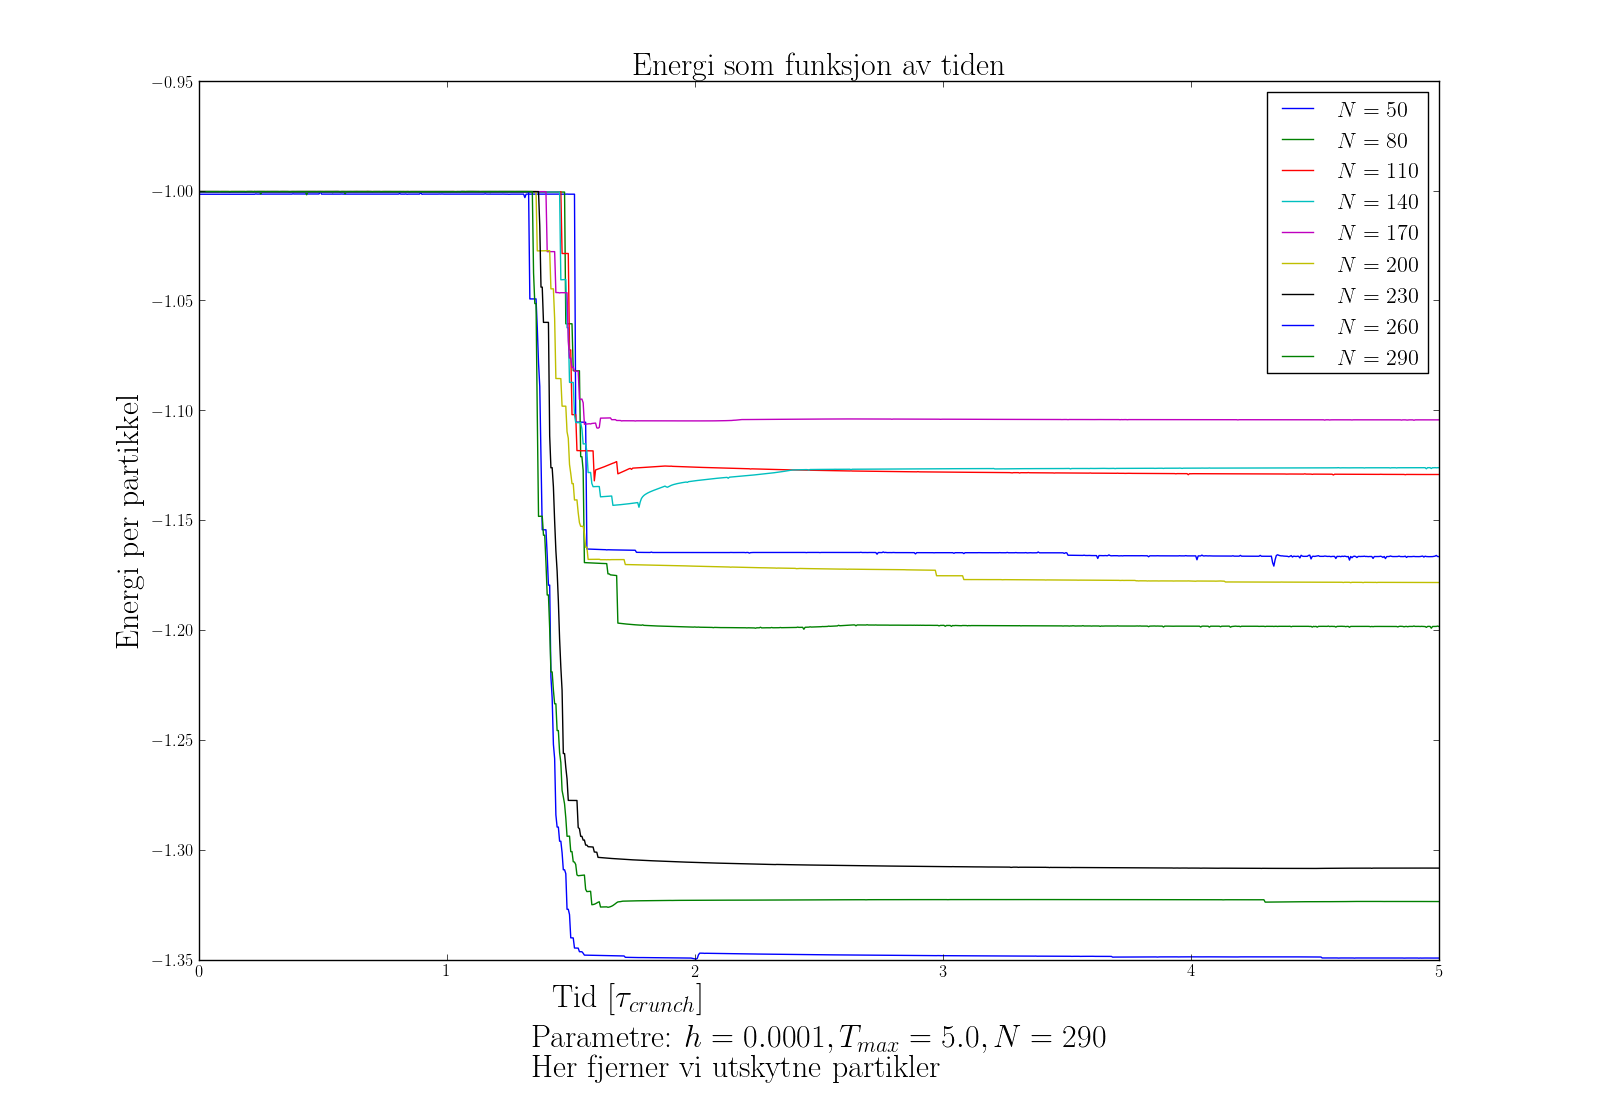
\includegraphics[width=\textwidth]{../fig/energy_plot_with_ejection_many_N.png}
  \caption{\label{fig:energy-many-N} Tidsforløpet til systemenergien
    for flere verdier av $N$. Vertikal akse er normalisert mot
    initialenergien for hver $N$. Vi ser at likevekten etableres mer eller
  mindre like fort uavhengig av hvor mange partikler som er med.}
\end{figure}
\begin{multicols}{2}



\subsection{Viralteoremet}
En interessant ting å se på er distribusjonen av kinetisk- og
potensiell energi. Viralteoremet sier noe om akkurat dette~\cite{viralteoremet-wiki}:

\begin{viralthm}
  For et gravitasjonelt bundet system i likevekt har vi 
\begin{align}
  2\mean{K} = -\mean{V}
\end{align}
\end{viralthm} 

\end{multicols}
\begin{figure}[!ht]
  \centering
  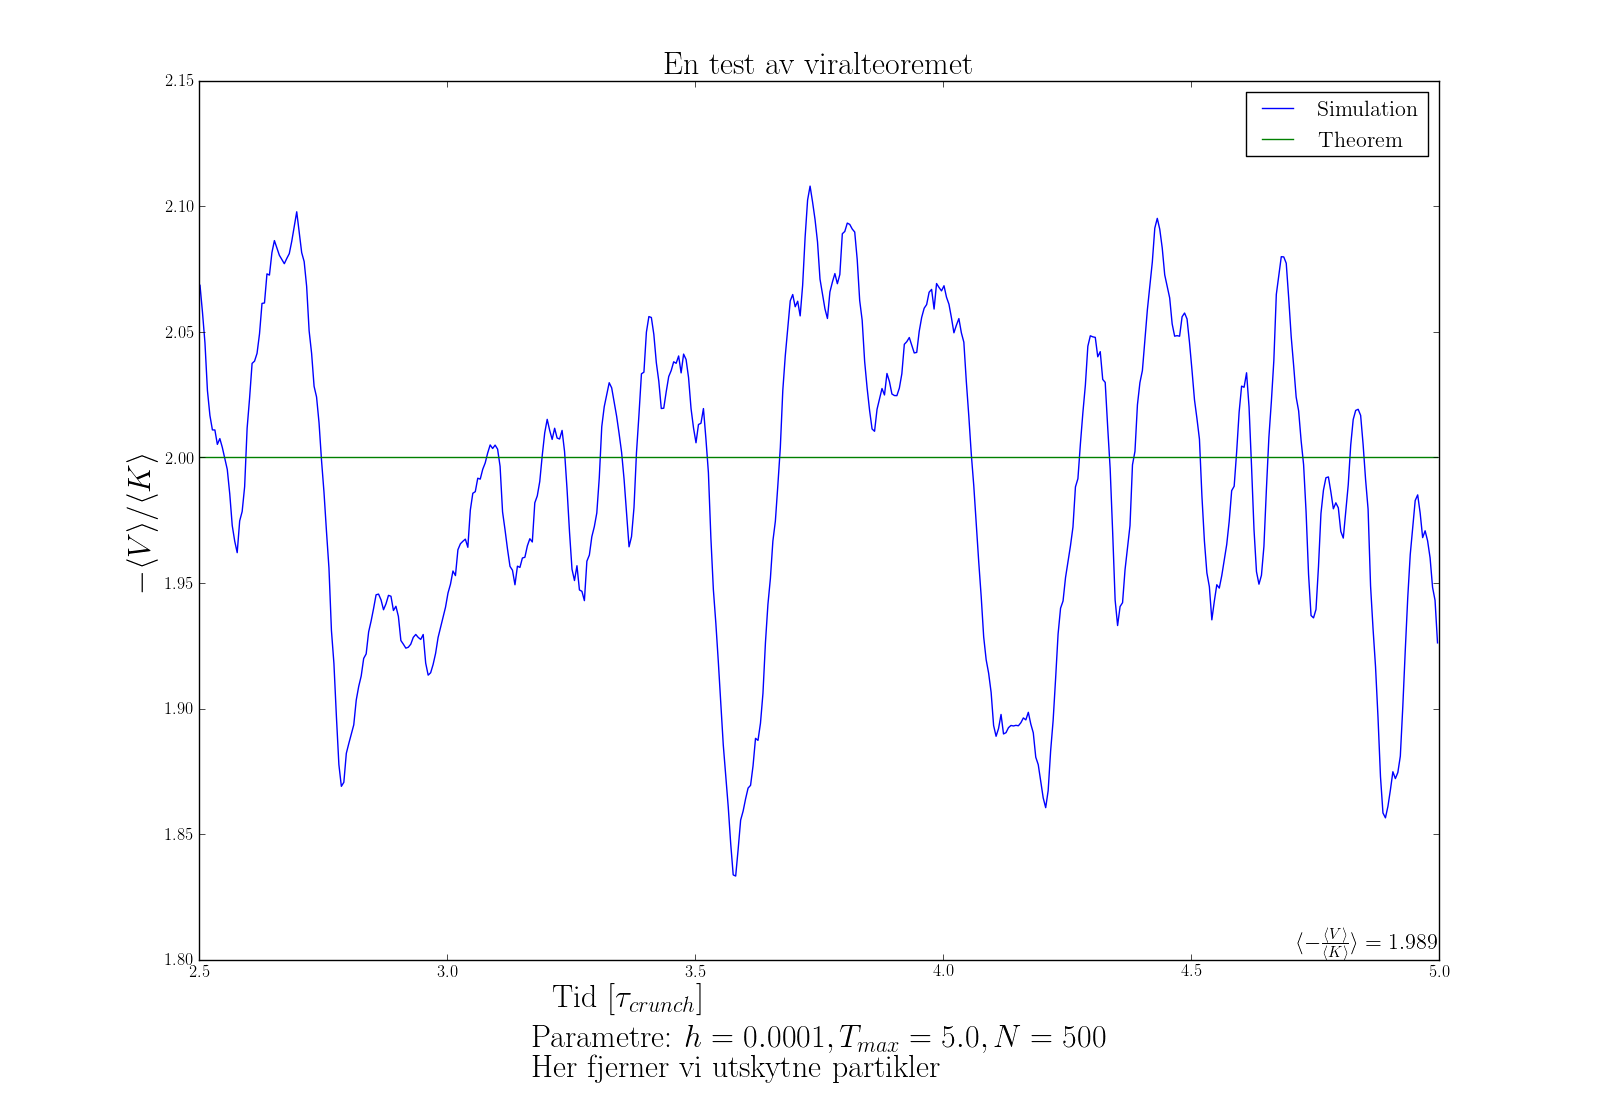
\includegraphics[width=\textwidth,height=300px]{../fig/viral.png}
  \caption{\label{fig:viral} Forholdet mellom potensiell- og kinetisk
 energi etter at vi har nådd likevekt. Figuren viser både tidsforløpet
til fordelingen og tidsmidlet. Vi ser at vi får en verdi som ligger
svært nære den verdien vi forventer fra Viralteoremet.}
\end{figure}
\begin{multicols*}{2}

Figur \ref{fig:viral} viser en graf av forholdet mellom potensiell- og
kinetisk energi etter at vi har nådd likevekt.\footnote{Plottet er
  laget med et program kalt
  \texttt{viralTheorem.py}~\cite{github-repo}} Det ser ut som om
forholdet i simuleringen oscillerer rundt den ideelle verdien fra
Viralteoremet. I høyre hjørne i figuren er tidsmidlet av forholdet
regnet ut, og som vi ser får vi en verdi svært nære 2. 

Vi har beregnet resultatene i figur \ref{fig:viral} ved å ta midlet av
alle partiklenes energi på et gitt tidspunkt. Dette kan vi gjøre ved
den ergodiske hypotesen~\cite{ergodisk-hypotese}. Tidsmidlet av disse
verdiene (tidsmidlet av partikkelmidlet) er det som er vist i høyre
hjørne på figuren.

Dette er oppløftende resultater, fordi det tyder på at systemet vårt følger
naturens lover på tross av de forenklingene som har blir
gjort. F.eks. styrker dette begrunnelsen for vårt valg av $\epsilon$
(seksjon \ref{sec:forste-test-epsilon}) ikke har gitt urealistiske
resultater. 




\end{multicols*}
\clearpage
\printbibliography
\clearpage
\section{Vedlegg}
\begin{itemize}
  \item[]\lstinputlisting[language=c++, caption={C++ metode som bruker Velocity Verlet til å tidsutvikle systemet.}, label={lst:solver-RK4}]{solversnippet.txt}
\end{itemize}

\end{document}
%%% Local Variables:
%%% mode: latex
%%% TeX-master: t
%%% End:
